\documentclass[12pt]{report}
\usepackage{graphicx}
\usepackage{titling}
\usepackage[latin1]{inputenc}
\usepackage{enumerate}
\usepackage{float}
\usepackage{latexsym}
\usepackage{amssymb}
\usepackage{amsthm}
\usepackage{amsfonts}
\usepackage[usenames,dvipsnames,svgnames,table]{xcolor}
\usepackage{listings}
\parindent=0pt
\frenchspacing
\pagestyle{empty}

\lstdefinestyle{prismmodel}{
	tabsize=1,
	captionpos=b
  	belowcaptionskip=1\baselineskip,
  	breaklines=true,
  	frame=single,
	frameround=tttt,
	captionpos=b,
  	language={},
  	numbers=left,
  	numbersep=5pt,
  	numberstyle=\tiny\ttfamily\color{Black},
  	basicstyle=\footnotesize\ttfamily\color{Black},
  	keywordstyle=\bfseries\color{Black},
	morekeywords={module, endmodule, label, init, mdp }, 
	otherkeywords={=, :, [, ], |},
	identifierstyle={\color{red}\let\textcolor\textcolordummy},
	morestring=[b][\color{red}\bfseries]",
	commentstyle=\color{Green},
	moredelim=[s][\color{DarkOrchid}\ttfamily]{[}{]},
	literate=%
		*{0}{{{\color{blue}0}}}1
	    {1}{{{\color{blue}1}}}1
	    {2}{{{\color{blue}2}}}1
	    {3}{{{\color{blue}3}}}1
	    {4}{{{\color{blue}4}}}1
	    {5}{{{\color{blue}5}}}1
	    {6}{{{\color{blue}6}}}1
	    {7}{{{\color{blue}7}}}1
	    {8}{{{\color{blue}8}}}1
	    {9}{{{\color{blue}9}}}1
}

\newcommand{\tab}[1]{\hspace{.2\textwidth}\rlap{#1}}
\newcommand{\HRule}{\rule{\linewidth}{0.5mm}}

\begin{document}

\begin{titlepage}
\begin{center}


\includegraphics[scale=2.0]{../GFX/dtu_logo.pdf}\\[1cm]

\textsc{\LARGE Technical University of Denmark}\\[1.5cm]

\textsc{\Large 02246 Model Checking}\\[0.5cm]


% Title
\HRule \\[0.4cm]
{\huge \bfseries Mandatory Assignment\\Part 1: Discrete Modelling and Verification}\\[0.1cm]
\HRule \\[1.5cm]

% Author and supervisor
\large
\emph{Authors:}
\\[10pt]
Andreas Hallberg \textsc{Kjeldsen}\\
\emph{s092638@student.dtu.dk}
\\[10pt]
Morten Chabert \textsc{Eskesen}\\
\emph{s133304@student.dtu.dk}

\vfill

% Bottom of the page
{\large October 21, 2013}

\end{center}
\end{titlepage}

\chapter*{HJ{\AE}LPE HALL{\O}J}
\begin{tabular}{ | l  c  r | }
	\hline
	CTL	& & Wiki \\ \hline
	$\forall$ & $\equiv$ &  A \\
	$\exists$ & $\equiv$ & E \\
	$\bigcirc$ & $\equiv$ & X \\
	$\Box$ & $\equiv$ & G \\
	$\Diamond$ & $\equiv$ & F \\
	\hline
\end{tabular}
\newpage

\chapter*{Part A: Introductory Problems}
\section*{A1) Practical Problems}

\subsection*{A1.1}
For the FCFS scheduler, we would like to verify that whenever a client has an active job, the scheduler has that job somewhere in its queue. For example, in the case of the first client, we require that whenever $state_1 = 1$, then either $job_1 = 1$ or $job_2 = 1$.

\subsubsection*{A1.1a) Express this as two CTL properties - one for each client}
$client_1$: $AG (state_1 = 1 \Rightarrow \neg(\neg job_1 = 1 \wedge \neg job_2 = 1))$\\
$client_2$: $AG (state_2 = 1 \Rightarrow \neg(\neg job_1 = 2 \wedge \neg job_2 = 2))$

\subsubsection*{A1.1b) Use PRISM to verify whether these properties hold of the FCFS scheduler model}
$P>=1 [G state1=1=>(job1=1)|(job2=1)]$ - Verified.\\
$P>=1 [G state2=1=>(job1=2)|(job2=2)]$ - Verified.

\subsubsection*{A1.1c) Write down two similar properties for the SRT scheduler, explaining your construction}
$client_1$: $AG (state_1 = 1 \Rightarrow job_1 = true)$\\
$client_2$: $AG (state_2 = 1 \Rightarrow job_2 = true)$\\
\\
We require that whenever $state_1 = 1$ then $job_1 = true$ because there should be a job waiting in the queue when the $state_1 = 1$. The same goes for $client_2$.

\subsubsection*{A1.1d) Verify whether they hold of the model}
$P>=1 [G state1=1=>job1=true]$ - Verified.\\
$P>=1 [G state2=1=>job2=true]$ - Verified.


\subsection*{A1.2}
Add another client to the PRISM model of the FCFS scheduler. You will need to modify the $Scheduler$ module to cope with the extra client, but for now do not increase the length of the queue.

\subsubsection*{A1.2a) Explain the changes that you made to the model, and argue why they satisfy the above instructions}
In order for the \emph{Scheduler} to cope with an extra client we first add an extra module called $client_3$ with the same commands as the two other clients with the names of the commands corresponding to $client_3$. We changed the finite range, which $job_1$ and $job_2$ can take their value over to 0\dots3. This does not increase the length of the queue because there is still only two jobs allowed in the queue ($job_1$ and $job_2$). We also added commands create3, serve3 and finish3 and only changed the values according to the number of $client_3$.

\subsubsection*{A1.2b) How many reachable states are in the new model?}
In the new model there are 214 reachable states.

\subsubsection*{A1.2c) What will happen if the queue is full when a client attempts to create a job?}
A client cannot create a job when the queue is full. This is because all the modules synchronize over all action names that appear syntactically in the modules. The commands create1, create2 and create3 are also in scheduler with a guard that specifies that the $job_2 = 0$ for creation of a job to be possible, and $job_2 = 0$ is only true if the queue is empty.

\subsubsection*{A1.2d) Do the properties you have previously verified still hold of the model? If not, why not?}
Yes the properties previously verified still hold in the new model. They do because the clients' states will only be 1 if their job is in the scheduler since the modules are synchronized.

\subsection*{A1.3}
Now modify the $Scheduler$ module so that the queue is of length three.

\subsubsection*{A1.3a) Explain the changes that you made to the model, and argue why they are correct.}
In order to modify the queue to have a length of three we add another job to the queue called $job_3$ which will hold the third job of the queue. We also changed the create commands to have the guard $job_3 = 0$ because now this is the last job in the queue, so when it is 0 there is a place for one more job. Furthermore we added another method for shifting the queue when there is an empty slot. The old command stays in place, but there is now another command with the guard $job_2=0$ \& $job_3>0$ that shifts $job_3$ to $job_2$ so it is moved up in the queue. Since the commands have no action names the commands can always occur \emph{independently} of what any other modules in the systems are doing - just so long as its guard is true.

\subsubsection*{A1.3b) How many reachable states are in the new model?}
In the new model there are 1459 reachable states.

\subsubsection*{A1.3c) Do the properties now hold of the model? If not, why not?}
The properties previously verified do not hold in the new model, because the queue is now of length 3. Which means that a job created by a client could be in scheduled as the last job, i.e. in $job_3$. Example: this would cause (for $client_1$) to have $state_1 = 1$ while $job_3=1$ because the job is at the end of the queue.

\subsubsection*{A1.3d) Can you give an upper bound on the number of reachable states for a model with $n$ clients, and a queue of length $m$?}
????????????????????????????

\subsection*{A1.4}
Consider the CTL properties $\Phi$ and AG $\Phi$, where $\Phi$ is an atomic property.

\subsubsection*{A1.4a) What are their semantics, and how do they differ?}
$AG$ $\Phi$ specifies that from all the paths from this state $\Phi$ should hold. Whereas property $\Phi$ should only hold in that state.

\subsubsection*{A1.4b) Are their semantics different in the version of PRISM that you use?}
The semantics are different in the version of PRISM we use. If the property $\Phi$ should hold in all reachable states it should be written $AG$ $\Phi$. Because if only $\Phi$ has been written as the property - this version of PRISM will only check if the property $\Phi$ holds in the \emph{initial} state.

\subsubsection*{A1.4c) How would you solve the classical model checking problem $M,s \models \Phi$ as a problem of the form $\forall s' : M,s' \models \Phi'$?}
I'll have to think about this.

\subsubsection*{A1.4d) How would you solve the model checking problem $\forall s' : M,s \models \Phi$ as a problem of the form $M,s' \models \Phi'$}
I'll also have to think about this.

\section*{A2) Theoretical Problems}
\subsection*{A2.1}
\begin{figure}[H]
	\centering
	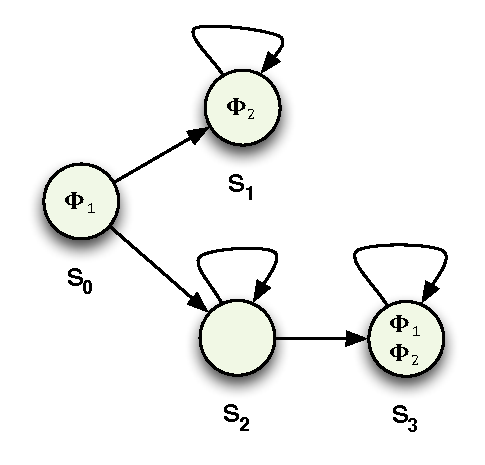
\includegraphics[scale=0.75]{../GFX/ExerciseFigure1.pdf}
	\caption{A transition system}
\end{figure}

Consider the transition system, shown graphically in \textbf{Figure 1}. The states are represented by circles, whose names are shown beneath them, and whose labels are shown inside them. The initial state is $s_0$.

\subsubsection*{A2.1a) Write down this transition system formally, as a tuple\\$(S,\rightarrow,S_0,AP,L)$}
The transition system will formally be written as:\\
$\langle\{s_0,s_1,s_2,s_3\},\{(s_0 \rightarrow s_1),(s_1 \rightarrow s_1),(s_0 \rightarrow s_2),(s_2 \rightarrow s_2),(s_2 \rightarrow s_3)\},s_0,\\
\{\Phi_1,\Phi_2\},\{(s_0, \{\Phi_1\}), (s_1, \{\Phi_2\}), (s_2, \{\}), (s_3, \{\Phi_1, \Phi_2\})\}\rangle$

\subsubsection*{A2.1b) By directly reasoning with the semantics of CTL, determine whether the following properties hold of the state $s_0$}
\begin{enumerate}[i.]
	\item $AF \Phi_2$: Does not hold as $s_2$ can loop infinitely and therefore $s_3$ is never reached.
	\item $AX \Phi_2$: Does not hold as $s_0 \rightarrow s_2$ isn't allowed.
	\item $EF \Phi_1$: Holds $(s_0 \rightarrow s_2 \rightarrow s_3$).
	\item $A[\Phi_1 U \Phi_2]$: Does not hold as $s_0 \rightarrow s_2$ isn't allowed.
\end{enumerate}

\subsection*{A2.2}
For each of the following pairs of CTL formulae, determine whether (a) they are equivalent, (b) one implies the other, or (c) neither implies the other. Explain your reasoning.
\begin{description}
	\item[A2.2a) $EX \; EF \; \Phi$ and $EF \; EX \; \Phi$:]
		They are equal\\
		$\left(EX \; EF \; \Phi \equiv EF \; EX \; \Phi\right)$.\\
		The first formulae dictates that somewhere there is a state which at some point has a descendant that contains $\Phi$. The second formulae dictates that somewhere there is a state which immediate descendant contains $\Phi$.
		\begin{figure}[H]
			\centering
			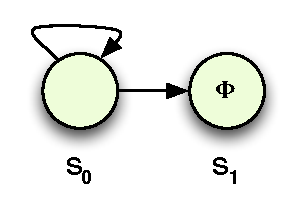
\includegraphics[scale=0.75]{../GFX/Answer-A2-2a.pdf}\\
			Figure A2.2a: A transition system.
		\end{figure}
		In Figure A2.2a both formulae will be satisfied. For the first formulae we match $s_0$ with $EX$ then somewhere in the descendant path of $s_0$ we reach $s_1$ which satisfies $EF \; \Phi$. For the second formulae we keep staying in $s_0$ for however long it might be and the final time we hit $s_0$ we will match $EF$ then immediately afterwards we will go to $s_1$ which satisfies $EX \; \Phi$.
		
	\item[A2.2b) $AX \; AF \; \Phi$ and $AF \; AX \; \Phi$:]
		They are equal\\
		$\left(AX \; AF \; \Phi \equiv AF \; AX \; \Phi\right)$.\\
		The first formulae dictates that for every state all the descendant states of the immediate descendant must somewhere have a state that contains $\Phi$. The second formulae dictates that all states must have a descendant which all immediate descendants contains $\Phi$.
		\begin{figure}[H]
			\centering
			\begin{tabular}{ l r }
				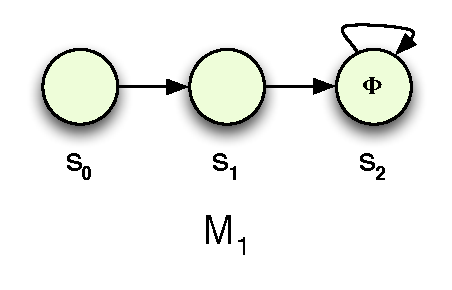
\includegraphics[scale=0.75]{../GFX/Answer-A2-2b-1.pdf}
				& 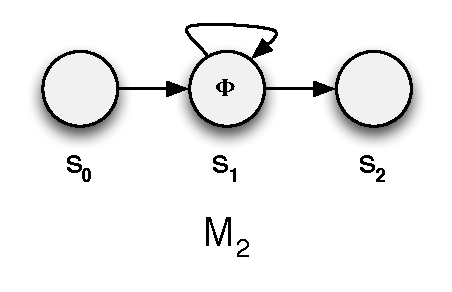
\includegraphics[scale=0.75]{../GFX/Answer-A2-2b-2.pdf}
			\end{tabular}\\
			Figure A2.2b: Two transition systems $M_1$ and $M_2$.
		\end{figure}
		In Figure A2.2b the transition system $M_1$ satisfies both formulae. Transition system $M_2$ will not satisfy any of the formulae as state $s_2$ will never be satisfied.
	
	\item[A2.2c) $AG \; EF \; \Phi$ and $EF \; AG \; \Phi$:]
		The first formulae implies the second formulae $\left(AG \; EF \; \Phi \Rightarrow EF \; AG \; \Phi\right)$.\\
		If $AG \; EF \; \Phi$ satisfies a transition system then $EF \; AG \; \Phi$ will satisfy the same transition system, but not the other way around. Figure A2.2c shows two transition systems, $M_1$ and $M_2$. $M_1$ will satisfy both formulae whereas $M_2$ will only satisfy the second formulae.
		\begin{figure}[H]
			\centering
			\begin{tabular}{ l r }
				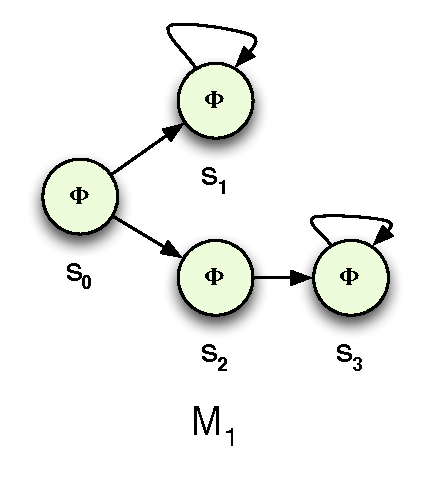
\includegraphics[scale=0.75]{../GFX/Answer-A2-2c-1.pdf}
				& 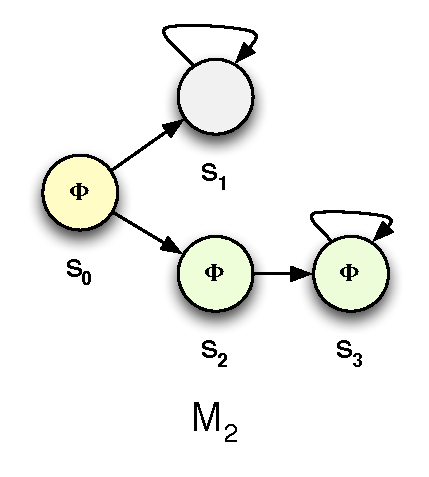
\includegraphics[scale=0.75]{../GFX/Answer-A2-2c-2.pdf}
			\end{tabular}\\
			Figure A2.2c: Two transition systems $M_1$ and $M_2$.
		\end{figure}
		\textcolor{ForestGreen}{Green} indicates a state that is satisfied for both formulae. \textcolor{Goldenrod}{Yellow} indicates a state that is satisfied by just the second formulae. \textcolor{Grey}{Grey} indicates a state that is satisfied by none of the formulae.
	
	\item[A2.2d) $AG \; (\Phi_1 \wedge \Phi_2)$ and $(AG \; \Phi_1) \wedge (AG\;\Phi_2)$:]
		They are equal\\
		$\left(AG (\Phi_1 \wedge \Phi_2) \equiv (AG \; \Phi_1) \wedge (AG \;\Phi_2)\right)$.\\
		The first formulae dictates that every state reachable must have $\Phi_1$ and $\Phi_2$. The second formulae firstly dictates that every state reachable must have $\Phi_1$ and secondly dictates that every state reachable must have $\Phi_2$. Thous for both of the formulae to be satisfied every reachable state must have both $\Phi_1$ and $\Phi_2$.\\
		Also it's a distribute law in CTL, see page 330 of the course book.
		
	\item[A2.2e) $EF \; (\Phi_1 \wedge \Phi_2)$ and $(EF \; \Phi_1) \wedge (EF \;\Phi_2)$:]
		The first formulae implies the second formulae $\left(EF \; (\Phi_1 \wedge \Phi_2) \Rightarrow (EF \; \Phi_1) \wedge (EF \;\Phi_2)\right)$.\\
		The first formulae dictates that there must exist a reachable state having both $\Phi_1$ and $\Phi_2$. The second formulae firstly dictates that there must exist a reachable state containing $\Phi_1$ and secondly it dictates that there must exist a reachable state containing $\Phi_2$. Thous if the first formulae is satisfied the second formulae must also be. On the contrary if the second formulae is satisfied the first formulae may not necessary also be, as $\Phi_1$ and $\Phi_2$ can be in different states but in the same tree, this would satisfy the second formulae but not the first.
		\begin{figure}[H]
			\centering
			\begin{tabular}{ l r }
				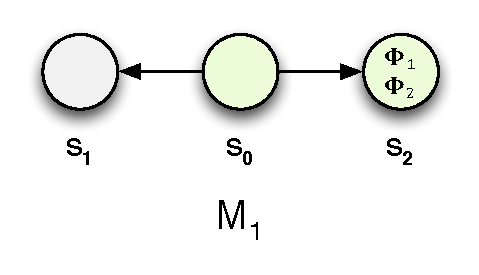
\includegraphics[scale=0.75]{../GFX/Answer-A2-2e-1.pdf}
				& 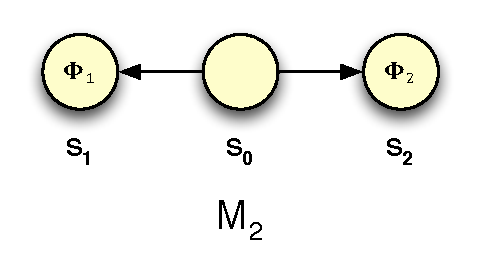
\includegraphics[scale=0.75]{../GFX/Answer-A2-2e-2.pdf}
			\end{tabular}\\
			Figure A2.2e: Two transition systems $M_1$ and $M_2$.
		\end{figure}
		\textcolor{ForestGreen}{Green} indicates a state that is satisfied for both formulae. \textcolor{Goldenrod}{Yellow} indicates a state that is satisfied by just the second formulae. \textcolor{Grey}{Grey} indicates a state that is satisfied by none of the formulae.
\end{description}

\subsection*{2A.3}
Write down a CTL* formula for each of the following properties, which are described in natural language. In each case, argue whether or not the property can also expressed in CTL.

\subsubsection*{2A.3a) There is a path on which $\Phi$ holds infinitely often}
	\textbf{CTL*:} $\exists \Box \Phi$\\
	\textbf{CTL:} Would be the same as for CTL*.

\subsubsection*{2A.3b) For all paths, $\Phi_1$ holds along the path until $\Phi_2$ holds of a state and $\Phi_3$ holds of the state that immediately follows}
	\textbf{CTL*:} $\forall (\Phi_1 U \Phi_2) \bigcirc \Phi_3$\\
	\textbf{CTL:} In CTL a path quantifier ($\exists, \forall$) has to be in front of a state operator ($\Diamond, \Box, \bigcirc, U, W$), therefore the formulae for CTL* is not possible to use with CTL. Furthermore, the CTL* formulae cannot be translated into CTL due to $\Phi_3$ having to follow $\Phi_2$ immediately. 

\subsubsection*{2A.3c) There is a path on which either $\Phi_1$ eventually holds or $\Phi_2$ eventually holds}
	\textbf{CTL*:} $\exists \Diamond \left((\Phi_1 \wedge \neg\Phi_2) \vee (\neg\Phi_1 \wedge \Phi_2)\right)$\\
	\textbf{CTL:} Would be the same as for CTL*.

\subsubsection*{2A.3d) For all paths, either $\Phi_1$ always holds or $\Phi_2$ always holds}
	\textbf{CTL*:} $\forall(\Box \Phi_1 \vee \Box \Phi_2)$\\
	\textbf{CTL:} Not possible to create due to the $\Box$ having to be inside the parentheses.

\newpage
\subsection*{2A.4}
Encode the transition system in \textbf{Figure 1} as a PRISM module, using a variable $s$, such that $0 \leq s \leq 3$, to represent the state. Define $\Phi_1$ and $\Phi_2$ as PRISM labels.\\
\\
\textbf{The PRISM module:}
\lstinputlisting[style=prismmodel,caption={PRISM module encoding the transition system in \textbf{Figure1}.}]{../A2.4.nm}

\chapter*{Part B: Intermediate Problems}
\section*{B1) Practical Problems}
\subsection*{Round-robin Scheduler}
In this part we will model a round-robin scheduler (found in the file RR.nm). A round-robin scheduler cycles between jobs and executes each task for just one time unit before moving onto the next. We model the scheduler by modifying the SRT scheduler which was handed out with the assignment (SRT.nm). In order to model a round-robin scheduler from the SRT scheduler we need to introduce some variables to the \emph{Scheduler} module.
\begin{center}
turn : {[0..2]} init 0; // Who is next?\\
job1time : bool init false; // Has job1 used up its time?\\
job2time : bool init false; // Has job2 used up its time?\\
\end{center}
The turn variable specifies which job is next to be served. When turn=1 the next job to be served is $job_1$ which is the job of $client_1$.\\
The $job_Xtime$ variable specifies if $job_X$ has used up all its serving time in the scheduler. So if $job_Xtime$ is true the next job should be served whereas if $job_Xtime$ is false this job should be served next. It should only be served next because there are only 2 jobs in this scheduler but if there were more jobs it should be served soon because it is not necessarily that job's turn next when more jobs are cycled.\\
We also introduce some new commands with no action names in the module. These commands can always occur independently of what any other modules in the system are doing. The guard of these commands just has to be true.
\begin{center}
{[]} job1=true \& job1time=true \& turn=1 $\Rightarrow$ (job1time$'$=false);\\
{[]} job2=true \& job2time=true \& turn=2 $\Rightarrow$ (job2time$'$=false);
\end{center}
These commands are used to cycle between the jobs. If $job_1$ has used up all its time in the scheduler but it is now $job_1$'s turn in the queue $job_1time$ should not be true because of the guard in the serve commands which we will look at next. It should then be modified to false so it can be served by the scheduler. The same goes for $job_2$.\\
The serve commands have been modified in order to be able to cycle the jobs in a round-robin fashion.
\begin{center}
{[serve1]} job1=true \& job2=false $\Rightarrow$ true;\\
{[serve2]} job1=false \& job2=true $\Rightarrow$ true;\\
{[serve1]} job1=true \& job2=true \& turn=1 \& job1time=false $\Rightarrow$ (job1time$'$=true) \& (turn$'$=2);\\
{[serve2]} job1=true \& job2=true \& turn=2 \& job2time=false $\Rightarrow$ (job2time$'$=true) \& (turn$'$=1);
\end{center}
It serves the jobs if there is no other job in the queue which is still intact from the model of the SRT scheduler. That should not be modified. However it should only serve a job if it is that job's turn to be served and the job has not used up its time being served. This is in the guard specified as turn has to correspond with the client's number and its jobtime has to be false.\\
We have also made some additions to the \emph{create} and \emph{finish} commands. The create command now has two different kinds for each client. One of the commands has the guard $job_X$=false and turn=0. This command is only used if there has not been any jobs scheduled in the round-robin scheduler before the creation of the new job. When turn=0 there has not been scheduled any jobs yet because turn is initialized as 0 and then turn is only altered between 1 and 2. The other create command is used when there has been created jobs previously which means that the turn variable has been used and therefore turn $>$ 0.
\begin{center}
{[create1]} job1=false \& turn>0 $\Rightarrow$ (job$1'$=true);\\
{[create1]} job1=false \& turn=0 $\Rightarrow$ (job$1'$=true) \& (turn$'$=1);\\
{[create2]} job2=false \& turn>0 $\Rightarrow$ (job$2'$=true);\\
{[create2]} job2=false \& turn=0 $\Rightarrow$ (job$2'$=true) \& (turn$'$=2);\\
$\dots$\\
{[finish1]} job1=true $\Rightarrow$ (job$1'$=false) \& (job1time$'$=false);\\
{[finish2]} job2=true $\Rightarrow$ (job$2'$=false) \& (job2time$'$=false);
\end{center}
The finish commands has been altered to also set the variable $job_Xtime$ to false. Since the job is now finished its time in the queue should not be specified as used up. It should therefore be sat as false so it does not affect the next job created by the same client.\\
This model of a round-robin scheduler has 277 reachable states.\\
We have specified some properties in CTL which we previously have verified for the FCFS and SRT schedulers. We will verify these properties in PRISM.\\
$client_1$: $AG (state_1 = 1 \Rightarrow job_1 = true)$\\
$client_2$: $AG (state_2 = 1 \Rightarrow job_2 = true)$\\
$client_1$: $AG(task_1>0 \Rightarrow AF task_1 = 0)$ \\
$client_2$: $AG(task_2>0 \Rightarrow AF task_2 = 0)$ \\

\subsection*{Priority First Come First Served Scheduler}
In this part we will model a FCFS scheduler that is able to handle tasks with two different priority levels. A FCFS scheduler serves a job until it is finished however this variant can stop a job if a new job is created with higher priority. In order to accommodate jobs having a priority the \emph{Client} module have to be modified to have an additional variable called \emph{priority} which can be either 1 or 2. When the priority is 2 the job has a higher priority than a job with priority 1. The create commands have been altered to 10 new ones so the client is able to create jobs with both priority 1 and priority 2.
\begin{center}
priority1 : [1..2] init 1; // Priority of the job\\
{[create1]} state1=0 $\Rightarrow$ (state1$'$=1) \& (task1$'$=1) \& (priority1$'$=1);\\
$\dots$\\
{[create1]} state1=0 $\Rightarrow$ (state1$'$=1) \& (task1$'$=1) \& (priority1$'$=2);\\
$\dots$
\end{center}
The \emph{Scheduler} module is modified so that when a new job is created and it has a higher priority than a job in the queue it moves ahead of that job. This is done in the module by creating some new create commands in the Scheduler module.
\begin{center}
{[create1]} job2=0 $\Rightarrow$ (job2$'$=1);\\
{[create2]} job2=0 $\Rightarrow$ (job2$'$=2);\\
{[create1]} job2=0 \& priority1=2 \& priority2=1 $\Rightarrow$ (job2$'$=job1) \& (job1$'$=1);\\
{[create2]} job2=0 \& priority2=2 \& priority1=1 $\Rightarrow$ (job2$'$=job1) \& (job1$'$=2);
\end{center}
When a new job is created by any of the clients and it has a priority of 2 and the existing job in the queue has a priority of 1 then the new job moves ahead in the queue and the existing job moves back. If the priorities of the jobs are the same no changes should be made and likewise when the existing job in the queue has a priority of 2 and the newly added job has a priority of 1 then no changes should be made. This however involves pre-empting. If a job is running and a job is created with a higher priority it will interrupt the running job and the new job will jump ahead in the queue. This can result in starvation of a job meaning that a job will never be served which will also mean that the client who created that job will never be able to create a new job. This model of FCFS with priority has 360 reachable states.\\
We have specified some properties in CTL which we previously have verified for the FCFS and SRT schedulers. We will verify these properties in PRISM.\\
$client_1$: $AG (state_1 = 1 \Rightarrow \neg(\neg job_1 = 1 \wedge \neg job_2 = 1))$\\
$client_2$: $AG (state_2 = 1 \Rightarrow \neg(\neg job_1 = 2 \wedge \neg job_2 = 2))$\\
$client_1$: $AG(task_1>0 \Rightarrow AF task_1 = 0)$ \\
$client_2$: $AG(task_2>0 \Rightarrow AF task_2 = 0)$ \\

The two last properties fail because this model could result in starvation of a job as explained earlier. This means that a job's length (which is specified in the variable task) will never reach 0.

\section*{B2) Theoretical Problems}
\subsection*{B2.1}

\begin{figure}[H]
	\centering
	\begin{tabular}{ l r }
		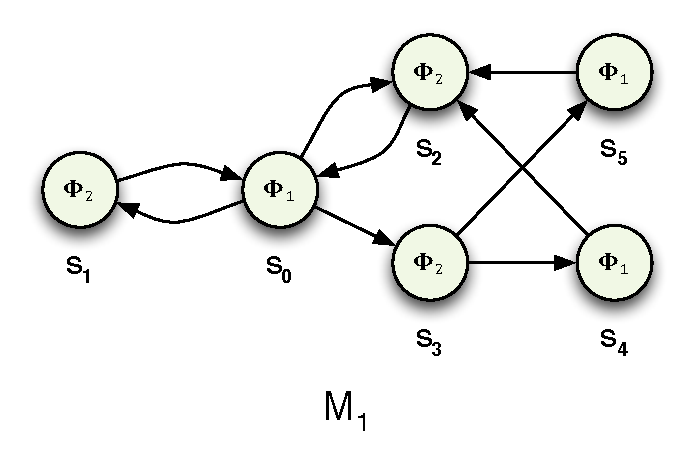
\includegraphics[scale=0.75]{../GFX/ExerciseFigure2-M1.pdf}
		& 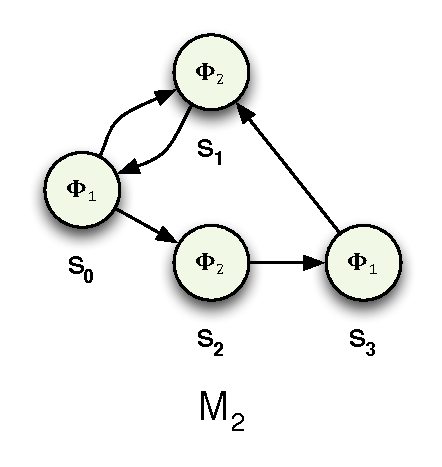
\includegraphics[scale=0.75]{../GFX/ExerciseFigure2-M2.pdf}
	\end{tabular}
	\caption{Two transition systems, $M_1$ and $M_2$}
\end{figure}
The two transition systems in Figure 2: $M_1 = (S_1,\rightarrow_1,\{s_0\},AP,L_1)$ and $M_2 = (S_2,\rightarrow_2,\{s_0\},AP,L_2)$ where $AP = \{\phi_1, \phi_2\}$.\\
We have to find the coarsest bisimulation relation between the states of the two structures: $R_{12} \subseteq S_1 \times S_2$.\\
The first step to find this is finding the states that have the same labels. This gives us:\\
$R_{12} = \{(s_0, s_0), (s_0, s_3), (s_1,s_1), (s_1,s_2),(s_2,s_1),(s_2,s_2),(s_3,s_1),(s_3,s_2),\\
(s_4,s_0),(s_4,s_3),(s_5,s_0),(s_5,s_3)\}$\\
The next step in finding the coarsest bisimulation relation between two transition systems is to remove the entries that does not satisfy the mutual simulation conditions. Doing so will give us the following:\\
$R_{12} = \{(s_0, s_0), (s_0, s_3), (s_1,s_1), (s_1,s_2),(s_2,s_1),(s_2,s_2),(s_3,s_1),(s_3,s_2),\\
(s_4,s_0),(s_4,s_3),(s_5,s_0),(s_5,s_3)\}$\\
$R_{12}$ is a bisimulation relation of $M_1$ and $M_2$ ($M_1 \sim M_2$) because the initial states are bisimilar: $s_0 R s_0$. It is also the coarsest bisimulation relation because we started by finding all the states that have the same label and put them in the relation. Then we proceeded to remove the entries that does not satisfy the mutual simulation conditions which led us to removing none. We did not remove any entries because every state in the two transition systems that have the same label have an incoming edge to a state with another label and an outgoing edge to a state with another level. 
\subsubsection*{(a)}

\subsubsection*{(b)}

\subsubsection*{(c)}

\subsubsection*{(d)}

\subsubsection*{(e)}

\subsubsection*{(f)}

\subsection*{2.}
\subsubsection*{(a)}

\subsubsection*{(b)}

\subsubsection*{(c)}

\subsubsection*{(d)}

\chapter*{Part C: Advanced Problems}
\section*{Practical Problems}
In the practical part of part B we modeled a round-robin scheduler. In this part we have modified the scheduler to include priorities (the model can be found in the Weighted-RR.nm file). When a scheduler has to include priorities it is important to decide how these priorities should affect the scheduling of jobs. In our specification the scheduler chooses the job with the highest priority and it serves it till its finished. There is however one exception to this. If a job has waited 5 turns this job will be served even though it may have a priority lower than the job that has been put on hold. This is a very simple but not a very convenient way to avoid starvation of a job because this could keep a job with a higher priority in the queue while serving a less important job. If the priority is equal the scheduler cycles between the jobs in a regular round-robin fashion. We use the notion that a job can either have a priority of 1 or 2 where 2 is the highest priority. This is specified by the client when the client creates a job. The \emph{Scheduler} module has been changed to accommodate priorities. It introduces two new variables $wait_1$ and $wait_2$ which specifies how long a job has waited and it is an integer between 0 and 5 with an initial value of 0. $wait_1$ specifies how long $job_1$ has waited and $wait_2$ specifies how long $job_2$ has waited.\\
The finish commands has been altered to accommodate the wait variables because if a job has finished it should not affect the clients next job that the previous job waited 4 turns for its turn. So the variable is reset to 0.\\
\begin{center}
{[finish1]} job1=true $\Rightarrow$ (job1$'$=false) \& (job1time$'$=false) \& (wait1$'$=0);\\
{[finish2]} job2=true $\Rightarrow$ (job2$'$=false) \& (job2time$'$=false) \& (wait2$'$=0);
\end{center}
The serve commands have also been altered to comply with jobs having priorities and waiting time. However one thing that should not be changed is the fact that if only one client has a job in the scheduler that job should of course be served. This can be seen in the first two lines below.
\begin{center}
1. {[serve1]} job1=true \& job2=false $\Rightarrow$ true;\\
2. {[serve2]} job1=false \& job2=true $\Rightarrow$ true;\\
3. {[serve1]} job1=true \& job2=true \& turn=1 \& job1time=false \& priority1=priority2 \& wait2$<$5 $\Rightarrow$ (job1time$'$=true) \& (turn$'$=2);\\
4. {[serve2]} job1=true \& job2=true \& turn=2 \& job2time=false \& priority2=priority1 \& wait1$<$5 $\Rightarrow$ (job2time$'$=true) \& (turn$'$=1);\\
5. {[serve1]} job1=true \& job2=true \& wait1=5 $\Rightarrow$ (turn$'$=2);\\
6. {[serve2]} job1=true \& job2=true \& wait2=5 $\Rightarrow$ (turn$'$=1);\\
7. {[serve1]} job1=true \& job2=true \& priority1$>$priority2 \& wait2$<$5 $\Rightarrow$ (turn$'$=2) \& (wait2$'$=wait2+1);\\
8. {[serve2]} job1=true \& job2=true \& priority2$>$priority1 \& wait1$<$5 $\Rightarrow$ (turn$'$=1) \& (wait1$'$=wait1+1);
\end{center}
The first two conditions in every guard above are very simple - the two job's have be to true meaning both clients have a job in the scheduler. Line 3 and 4 specifies the regular round-robin. If the priorities are equal and a job has not waited 5 turns for its turn then they should be cycled in a regular round-robin fashion. Line 5 and 6 specifies that if one job has waited 5 turns then that job should be served until it is finished and then the wait variable is reset to 0. However the update in these lines are interesting it changes the turn variable so it is the other job's turn to be served. This is done so that when $job_1$ is finished and that $client_1$ enters another job with the same priority as $job_2$ it will be $job_2$s turn to be served. This is a minor detail done in order to faster clear out jobs in the scheduler. Line 7 and 8 serves a job if its priority is higher than the other job's priority and it the other job has not waited 5 turns. The update again changes the turn variable to the other job for the same reason as line 5 and 6. It also increments the wait variable for the other job so the other job does not have to wait too long to be served. The Weighted-RR model has 3655 reachable states.\\
We have specified some properties in CTL which we will use PRISM to verify for our model. The properties specified below can also be found specified in PRISM notation in the Weighted-RR.pctl file.\\
\begin{tabular}{ c c c }
\\No. & CTL & Verified \\
1. & $AG (state_1 = 1 \Rightarrow job_1 = true)$ & $\checkmark$ \\
2. & $AG (state_2 = 1 \Rightarrow job_2 = true)$ & $\checkmark$ \\
3. & $AG(task_1>0 \Rightarrow AF task_1 = 0)$ & $\checkmark$ \\
4. & $AG(task_2>0 \Rightarrow AF task_2 = 0)$ & $\checkmark$ \\
5. & $A(task_1>0 \wedge wait_1=5 U task1=0 \wedge job1=false$ & $\checkmark$ \\
6. & $AG(wait_1=5 \wedge task_1=1 \Rightarrow (AX task_1=0))$ & X \\
7. & $AG(wait_1=5 \wedge task_1=1 \Rightarrow (EX task_1=0))$ & $\checkmark$ \\
8. & $AG(wait_1=5 \wedge task_2=1 \Rightarrow (EX task_2=0))$ & X \\
9. & $AG(wait_2=5 \wedge task_1=1 \Rightarrow (EX task_1=0))$ & X \\
10. & $AG(priority_2>priority_1 \wedge task_2=1 \wedge wait_1<5 \Rightarrow (EX task_2=0))$ & $\checkmark$ \\
11. & $AG(priority_2>priority_1 \wedge task_2=1 \wedge wait_1<5 \Rightarrow (EX task_1=0))$ & X \\
\\
\end{tabular}
No. 1 is a property that specify that if $state_1$ is 1 then $job_1$ should be true meaning that when $client_1$ has created a job it should be in the scheduler. The same goes for $client_2$ which is specified by no. 2 in the list.\\
No. 3 and 4. specify that it is globally the case whenever $task_1$ and $task_2$ is larger than 0 then it should eventually hold that $task_1$ and $task_2$ is 0 which means that the job has to eventually finish. This property could not be verified if the scheduler did not avoid starvation because then a job would never finish and it would just be in the scheduler forever. We prevent this by having a maximum waiting period of 5 turns as explained earlier.\\
No. 5 specifies that when $job_1$ has waited 5 turns and the job's length is larger than 0 it should hold until $task_1$ = 0 and $job_1$ = false. This is a property to verify that when a job has waited 5 turns it should be served till it is finished.\\
No. 6 specifies that it is globally the case that if a job has waited 5 turns and the length of its job is only 1 then in all the next states the length of the job should be 0, i.e. the job is finished. This property has not been verified and it should not be because in the scheduler there are two actions that can happen independently of all the other modules and this could create a new state where some of the variables have changed.\\
No. 7 specifies that it is globally the case that if a job has waited 5 turns and the length of its job is only 1 then in one of the next states the length of job should be 0. This property has been verified. This verifies that in one of the next states it is the job's turn to be served when it has waited 5 turns, however this is not enough to verify that the job will always be served ahead of the other job because of its waiting period.\\
This brings us to no. 8 and 9. No. 8 and 9 specify that if a job has waited 5 turns and the length of the other job is 0 then in one of the next states the length of the other job should be 0. This is not verified by PRISM which means that it is modeled correctly. It means that if a job has waited 5 turns the other job will never be served ahead of that job.\\
No. 10 specifies that if a job has a higher priority than the other job and its length is 1 and the other job has not waited 5 turns then in one of the next states the length of the job should be 0. This has been verified by PRISM. It verifies that it in one of the next states it is the job's turn to be served when it has a higher priority than the other job. Again however this is not enough to verify that the job will always be served ahead of the other job if it has a higher priority and the other job has not waited 5 turns. \\
This brings us to no. 11. No. 11 specifies that if a job has a higher priority than the other job and its length is 1 and the other job has not waited 5 turns then in one of the next states the length of the other job should be 0. This is not verified by PRISM which means that it is modeled correctly. It means that if a job has a higher priority and the other job has not waited 5 turns the other job will never be served ahead of that job.
\end{document}
